% !TeX root = document.tex
% !TeX program = lualatex

% !TeX root = document.tex
\documentclass[tikz, border=10pt]{standalone}

\usetikzlibrary{quotes}


\begin{document}
\setlength{\unitlength}{1cm}
\begin{picture}(1,1)
	\put(0,0){\circle{1}}
	\put(-0.5,0){\line(1,0){1}}
	\put(-.3,.06){text}
\end{picture}
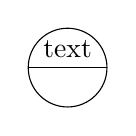
\begin{tikzpicture}
	\draw circle (0.5);
	\draw (-.5,0) to ["text"] (.5,0);
\end{tikzpicture}
\begin{tikzpicture}
	\draw[thin,dotted,step=0.5] (-3,-3) grid (3,3);
	\draw[->] (-3,0) -- (3,0);
	\draw[->] (0,-3) -- (0,3);
\end{tikzpicture}
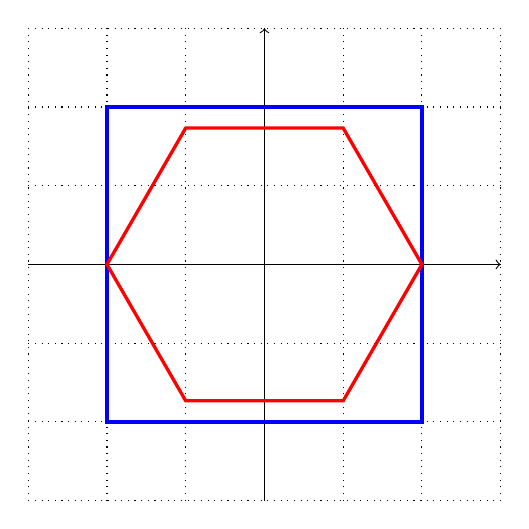
\begin{tikzpicture}
  \draw[thin,dotted] (-3,-3) grid (3,3);
  \draw[->] (-3,0) -- (3,0);
  \draw[->] (0,-3) -- (0,3);
  \draw[very thick, blue] (-2,-2) -- (-2,2)
    -- (2,2) -- (2,-2) -- cycle;
	\draw[very thick, red] (0:2) -- (60:2) -- (120:2)
	-- (180:2) --(240:2) -- (300:2) -- cycle;
\end{tikzpicture}
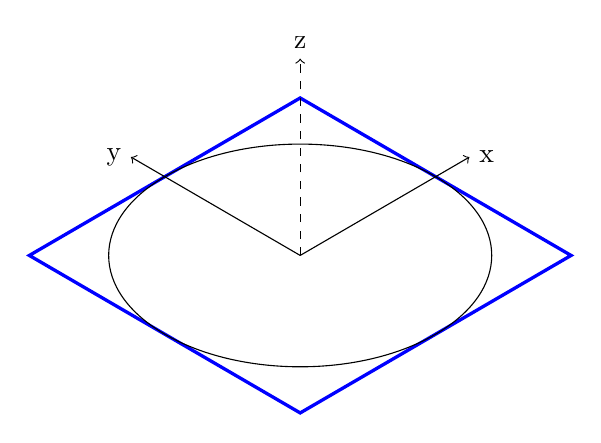
\begin{tikzpicture}[x={(0.86cm,0.5cm)},
  y={(-0.86cm,0.5cm)}, z={(0cm,1cm)}]
  \draw[very thick, blue] (-2,-2,0) -- (-2,2,0)
   -- (2,2,0) -- (2,-2,0) -- cycle;
  \draw[->] (0,0,0) -- (2.5, 0,  0) node [right] {x};
  \draw[->] (0,0,0) -- (0,  2.5, 0) node [left] {y};
  \draw[->,dashed] (0,0,0) -- (0,  0, 2.5) node [above] {z};
  \draw circle (2);
\end{tikzpicture}
\begin{tikzpicture}
	\draw[very thick, blue] (-3,-1) -- +(1,0)
  -- +(2,2) -- +(4,2) -- +(5,0) -- +(6,0);
	\draw[thin, dotted] (-3,-3) grid (3,3);
\end{tikzpicture}

\begin{tikzpicture}
	\draw[shading=ball, ball color=yellow] (0,0)
  circle [radius=2];
\draw[shading=ball, ball color=black] (-0.5,0.5,0)
  ellipse [x radius=0.2, y radius=0.4];
\draw[shading=ball, ball color=black] (0.5,0.5,0)
  ellipse [x radius=0.2, y radius=0.4];
\draw[very thick] (-1,-1) arc [start angle=185,
  end angle=355, x radius=1, y radius=0.5];
\end{tikzpicture}

\usetikzlibrary{datavisualization}
\begin{tikzpicture}
	\datavisualization [
		scientific axes=clean, 
		x axis = {
			attribute=batch_size, 
			ticks=many, length=\linewidth, label=batch size 
		},
		y axis = {
			attribute=time, 
			include value=0, 
			length=8cm, 
			label=time,
			ticks={tick unit=ns},
		},
		all axes={grid},
		visualize as scatter,
	] data [
		format=table, 
		read from file=data1.txt, 
		separator=\space,
		headline={batch_size time}
	];
\end{tikzpicture}

\end{document}
